\chapter{Introduction}
\label{chp:introduction}
The advances of positioning technologies are empowering a myriad of different objects present in our daily usage, e.g.
vehicles, smartphones and wearable devices, to be shipped with location tracking systems. Those devices are able to
collect and report mobility information of people, animals and natural phonemena (e.g. hurricanes), to name a few. That
technological advance is enabling the generation of massive volumes of spatio-temporal data that can contain information
ranging from the daily routine of residents of a city \citep{whatdidyoudo} to behaviors of wild animals in a specific
region \citep{trajclustering}\citep{miningperiodic}. It is notorious the interest of the academy in such subject,
specially with the rising of Smart Cities, in which spatio-temporal datasets can provide important insights in the
context of traffic management and urban planning \citep{gissmartcities}\citep{parallelsmartcities}. Those datasets can
be used to help solving a variety of problems and answer questions, such as:

\begin{enumerate}
    \item \textbf{What are the busiest times and locations (such as traffic jams locations) in a city?}
        \citep{visualtrafficjam}
    \item \textbf{What is the movement patterns of the citizens of a city during work hours?}
    \item \textbf{What is the migration pattern of inhabitants of a specific area?}
    \item \textbf{What is the movement behavior of wild animals in their habitat?} \citep{movemine}
    \item \textbf{Is there any suspicious movement of groups o objects during that time window?}
\end{enumerate}

That list can grow indefinitely, as the scenarios and applications of spatio-temporal data analysis is vast. Some of the
questions listed above are in the context of Smart Cities, which can take advantage of spatio-temporal data analysis as
an aid to a broad set of applications, like urban planning, public security, and public health and commerce
\citep{ieeesmartcities}. Aditionally, understanding that data and being able to take actions fast according to the
conclusions extracted from them is crucial to create and evolve a Smart City. However, due to the volume of data that is
produced on a daily basis and needs to be analyzed to in order to help those applications and answer those questions,
the main problem is still the same: how to be able to analyze massive data volumes fast and efficiently so we can
empower decision takers to act quickly?

In the aforementioned questions and applications, some of the queries are intrinsically related to collaborative or
group patterns, such as flock \citep{gudefficient}, convoy \citep{convoy}, swarm \citep{swarm}, and the like. Those
patterns contain moving objects that have a strong relationship by being close to each other, within a certain distance
range and during some minimum time interval. Due to the wide range of applicability in the scenario of Smart Cities
(e.g. city roads planning, intelligent transportation, public security, etc.), the data mining of such patterns has
gained great importance in both industry and academy. There are a number of research challenges in this topic, specially
regarding the development of accurate algorithms to detect those patterns. In addition of being precise, it is of
paramount importance to design fast algorithms so that they can be keep up with real-time data. Hence, reiterating what
as mentioned in the previous paragraph, efficiently extraction of data patterns for real-time analysis and on the fly
decision-making is still an open challenge.
% * <steniofernandes@gmail.com> 2016-05-26T15:01:34.895Z:
%
% gap: why individual tracking is not a good idea? in other words, why perform flock analysis in several contexts, including smart cities
%
% ^.

\begin{figure}[h!]
    \centering
    \caption{T1, T2 and T3 form a flock of size 3 with minimum length of three time steps, with a disk enclosing all
        trajectories at each time step}
    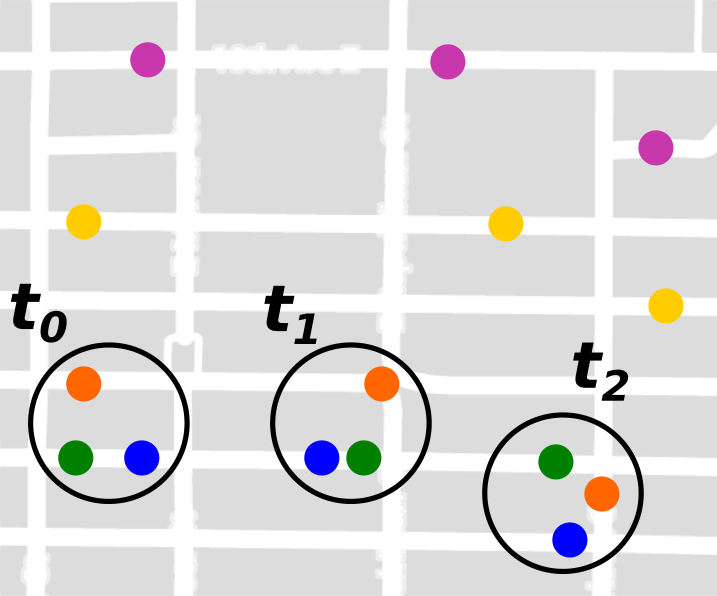
\includegraphics[width=0.7\linewidth]{images/flock_pattern.png}
    \footnotesize{Source: Made by the author.}
    \label{fig:flocks}
\end{figure}

Among those collaborative patterns, the flock pattern is one that has gained a lot of attention in the academy, since it
can address all the scenarios and questions that were mentioned in this chapter and represents a very familiar behavior
that is frequently seen in our daily routines. A seminal formal definition of that pattern was proposed by \citep{remo}
and \citep{gudefficient} and since then, a lot of other studies has follow suit (we refer the reader to
\chapref{chp:relatedwork} for some of them), mainly due to the interests in developing mechanisms to solve real-world
problems in the scope of Internet of Things (IoT) \citep{iot} and Smart Cities \citep{smartcities}.  According to
\citep{gudefficient}, a flock pattern consists of a minimum number of entities that are within a disk of radius
\textit{r} at a given time. However, this definition only applies to one single time step and does not help on
extracting some useful collective behavior information. Such initial definition was then extended by
\citep{gudreportingflock}, introducing the minimum time interval $\delta$ that the entities should stay together in
order to characterize a flock pattern, as depicted by \figref{fig:flocks}. The figure shows a flock pattern that lasts
three time steps and is formed by trajectories $T_1$, $T_2$ and $T_3$. It is worth mentioning that trajectories $T_4$
and $T_5$ are tno part of a flock pattern because there are no disks enclosing them in all three time steps.

When it comes to flock pattern detection efficiency and speed, one major problem on doing that is to find the disks that
enclose the trajectories in each time step. Since the disks centers do not need to match any point in the dataset, there
can be infinite possible disks. Vieira et al. \citep{vieira} proposed a way to limit the number of disks to generate and
analyze, so a finite number of disks are in place to cluster the trajectories in them. He also proposed an algorithm to
find the flock pattern, namely Basic Flock Evaluation (BFE). Even though BFE can find flock patterns in spatio-temporal
datasets, it does suffer from some severe performance limitations, meaning that it is not able to scale properly when
the dataset is really large. The main reason that we identified that makes it be so inefficient is that BFE it is not
smart enough to predict what portions of the data can really generate a flock patterns, then it ends up wasting
CPU cycles by processing data that is not important.

Despite the considerable number of research works in the academy regarding flock pattern detection, there is still a
problem that remains open, besides the fast pattern detection that we already mentioned: A framework/system architecture
for flock pattern detection that can be generalized to other data mining problems. In the systematic revision of the
the literature that we made in this field, we could not find any work formalizing a Software Architecture that can be
extensible, easy to use and still simple to address the pattern detection problem. By creating such Architecture,
researchers can take advantage of that as a starting point to develop their algorithms and can also have a common ground
to compare and reuse work of others.

As could be noticed, the state of the art algorithms for flock pattern detection are not ready to aid the development
and evolving of Smart Cities, since they are not able to efficiently process the huge volumes of data that are generated
by them. With that in mind, this dissertation proposes an efficient flock detection algorithm aiming at achieving
considerable gains in execution time, without compromising accuracy, thus targeting real-time deployment and online
processing. With that algorithm, we could address Smart Cities scenarios, where decisions need to be made on the fly and
rapidly enough in order to keep up with their development pace \citep{ieeesmartcities}\citep{springersmartcities}. Such
gains were made possible by creating a filtering heuristic, based on bitmaps, in order to save processing time. Our
proposal focuses on identifying Moving Objects (MO) that can actually form a flock, resulting in a huge reduction in the
number of disks generated and thus resulting in less data to be processed. Our results indicate that our proposal
outperforms the current state-of-the-art techniques, by achieving 99\% CPU time improvement and 96\% disks generation
reduction in some relevant scenarios. Going even further, we also remodeled our proposed algorithm to take advantage of
multi-core architectures, having some components executing in parallel resulting in impressive speed gains. With our
Multi-threaded model, we were able to reduce the processing time of our proposed algorithm by 96\% in some cases. It is
worth mentioning that the gains achieved with the Multi-threaded model are over the gains that we had already obtained
over the state-of-the-art techniques.

Last, but not least, we also propose a Generic System Archicture that can be used to solve a great number of data mining
problems. We validate our architecture by implementing our algorithm and our multi-threaded model using it as the
building blocks. Hence, to summarize, the contribution of this dissertation is threefold:

\begin{enumerate}
    \item \textbf{An effiecient flock pattern detection algorithm}
    \item \textbf{A remodeled algorithm able to take advantage of multi-core architectures and rapidly find flock
        patterns}
    \item \textbf{A simple and extensible System Archicture to aid solving spatio-temporal pattern detection problems}
\end{enumerate}

The remainder of this dissertation is organized as follows. \chapref{chp:relatedwork} highlights the related work in
both flock detection and trajectory data mining and exmplain in more details the academic contribution of our work.
\chapref{chp:techbackground} presents the technical background necessary to understand this dissertation, like the
formal Flock definition and how an algorithm to find a flock pattern works. Our contribution is detailed in
\chapref{chp:solution}, whereas in \chapref{chp:results} we show the results of our evaluations using our chosen
metrics. Lastly, in \chapref{chp:conclusion} we draw some concluding remarks and provide directions for future work.
